\newpage
\section*{Appendix}

\renewcommand{\thesection}{\Alph{section}}
\renewcommand\thefigure{S.\arabic{figure}}
\setcounter{figure}{0}
\renewcommand\thetable{S.\arabic{table}}
\setcounter{table}{0}



\begin{figure*}[t]
\centering
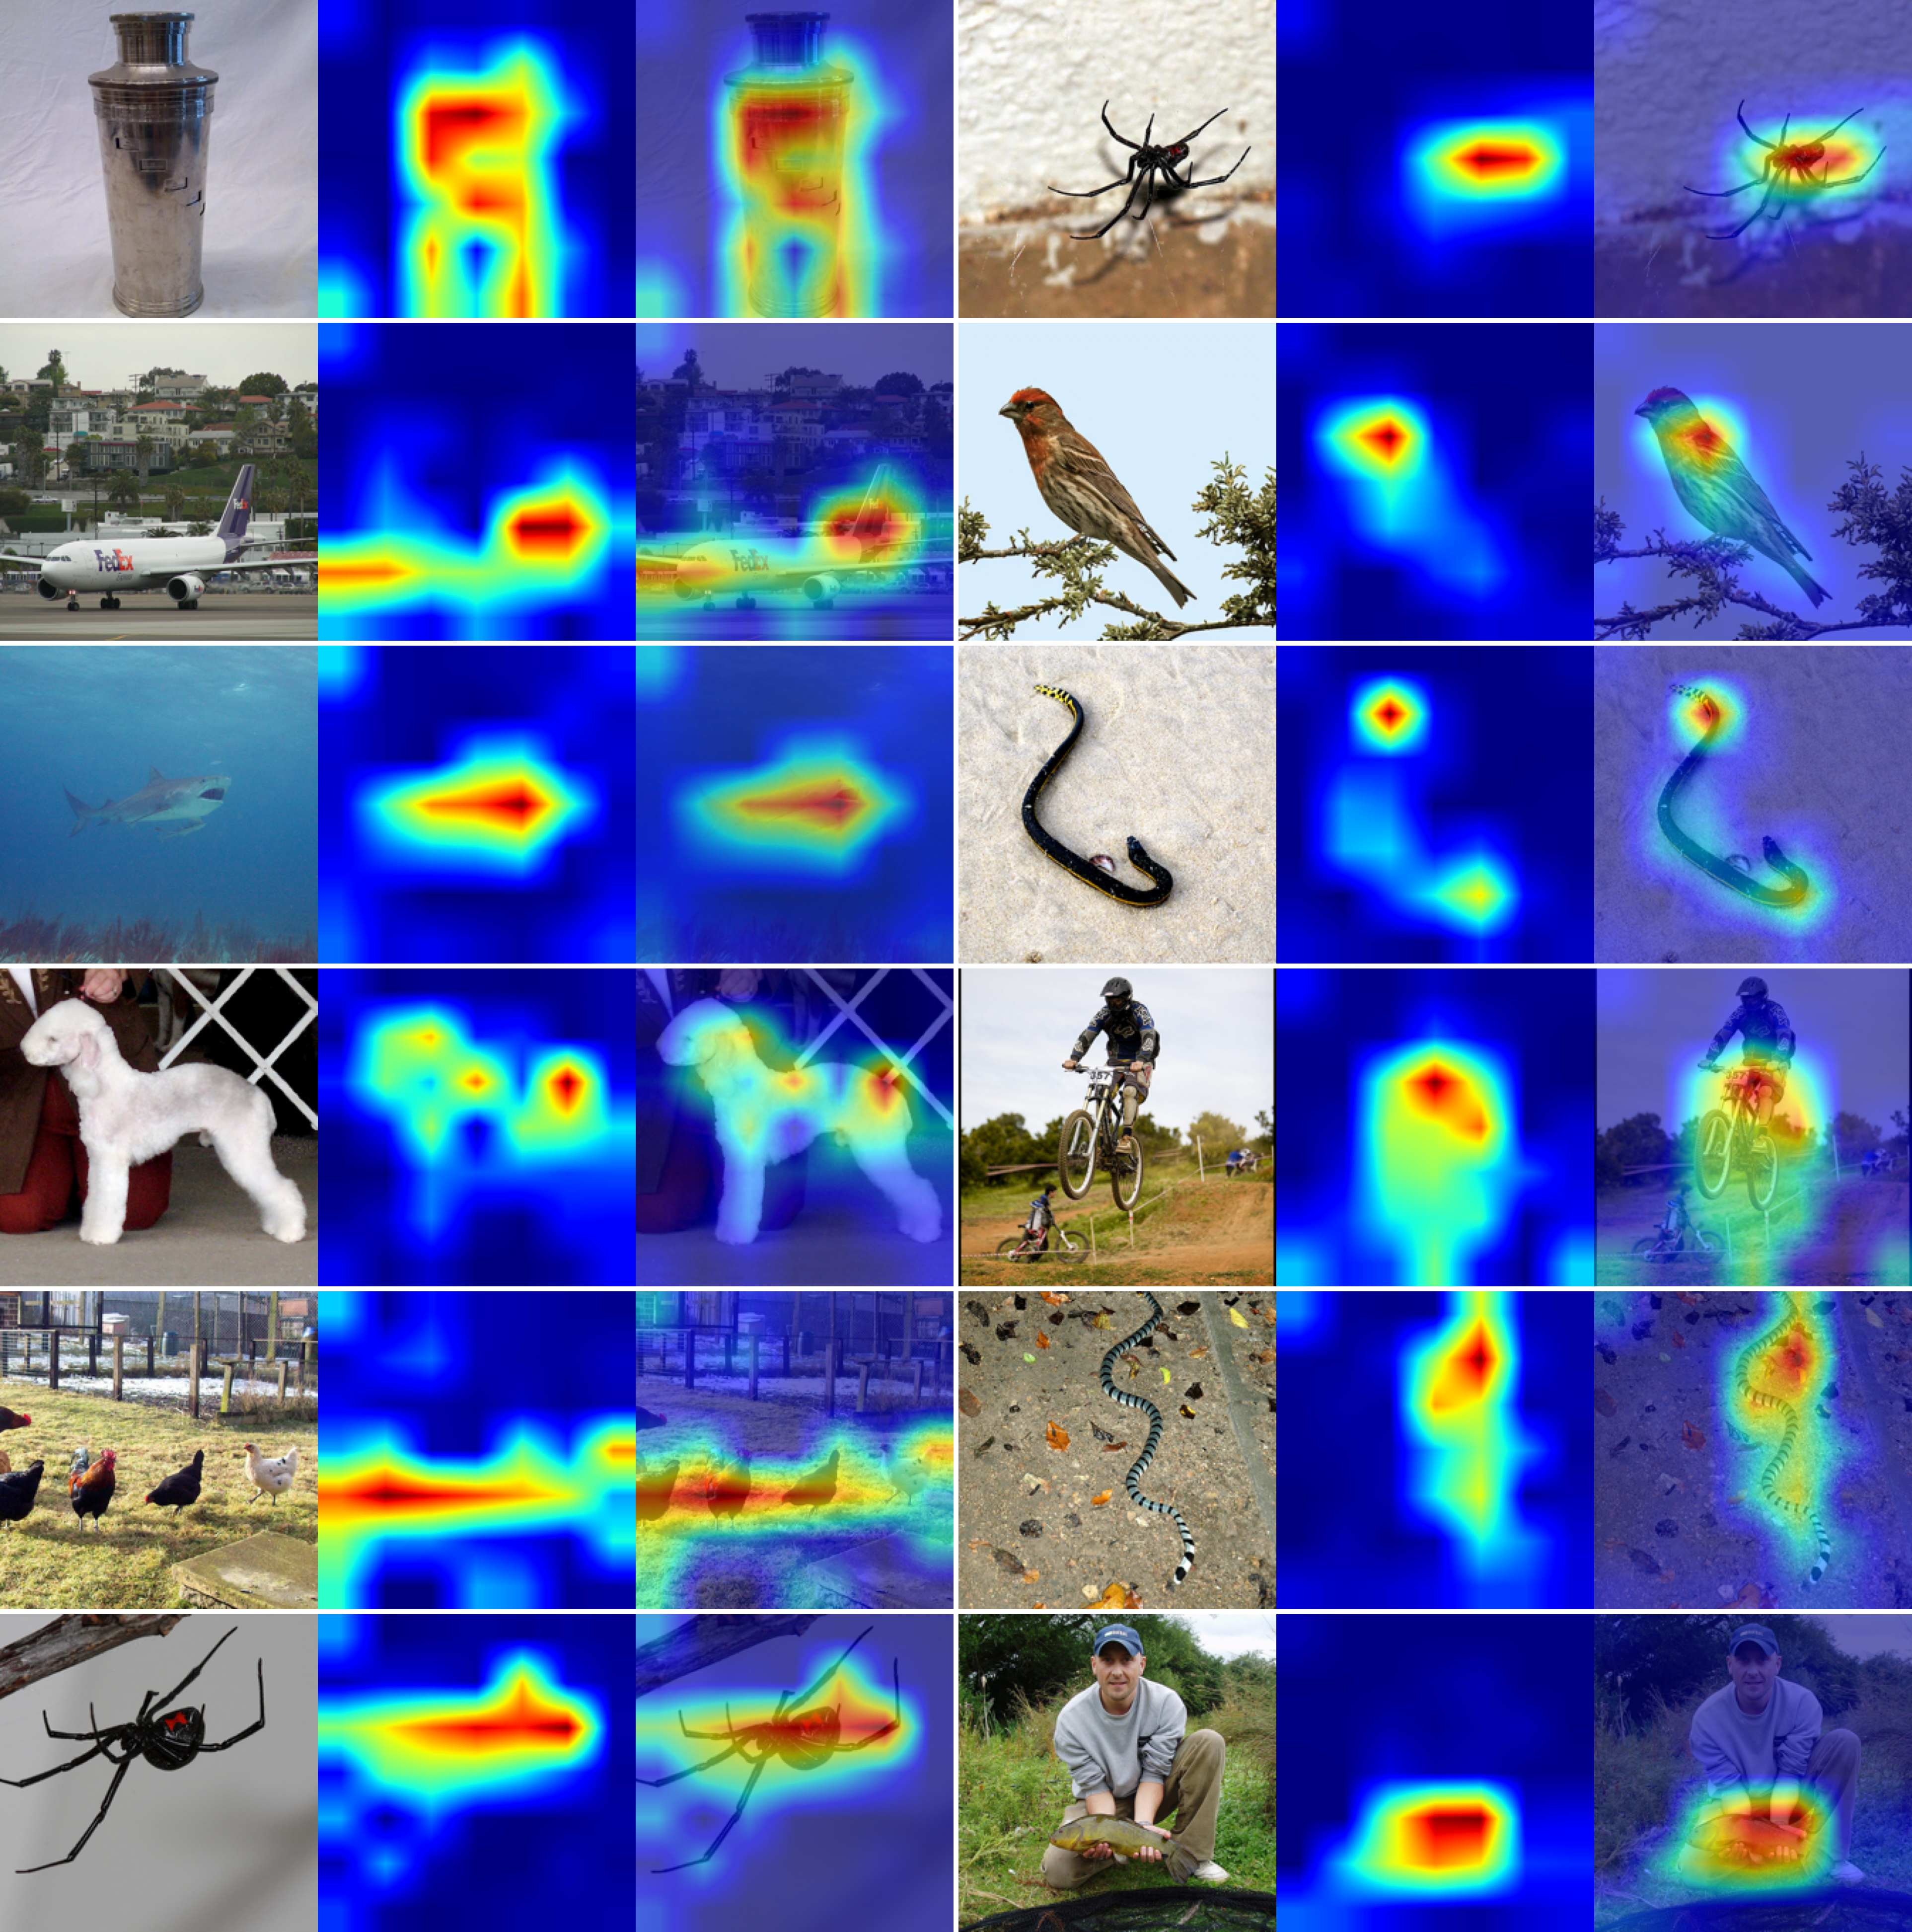
\includegraphics[width=\linewidth]{figures/abl_attn.png}
\caption{Visualization of MambaVision's attention patterns. Each row contains two example cases, with each case showing a triplet of: (left) original input image, (middle) attention heat map, and (right) attention overlay on the input image. The examples showcase diverse scenarios: containers and spiders (row 1), aircraft and birds (row 2), marine life and snakes (row 3), groomed dogs and extreme sports (row 4), poultry and snakes (row 5), and arachnids and outdoor activities (row 6). The attention maps reveal how MambaVision effectively localizes key semantic regions and object boundaries across this wide range of categories.}
\label{fig:attention_viz}
\end{figure*}


\section{Ablation Study}
To determine the optimal window size for MambaVision models, we study its impact on the performance of MambaVision-T in different tasks such as image classification, object detection and instance segmentation. Given $Q, K, V$ as the query, key and value tensors respectively, self-attention is computed according to
\begin{equation}
    {\rm Attention}({Q}, {K}, {V}) = {\rm Softmax}(\frac{{Q}{K}^\mathsf{T}}{\sqrt{d_{h}}}){V}.
    \label{eqn:mhsa_abl}
\end{equation}
$d_{h}$ represents the number of attention heads. If the input size is larger than the window size, the attention is computed in the local windows. Specifically, we study two different architectures with window sizes of 7 and 14 in their stage 3 of the model. We also measure image throughput for the task of image classification with a batch size of 128. As presented in Table~\ref{tab:abl_study_window}, our analysis reveals that increasing the window size to 14 offers a favorable trade-off between performance and computational cost. While maintaining nearly identical throughput (6298 img/s vs. 6318 img/s), the larger window size achieves consistent improvements across all vision benchmarks: ImageNet top-1 accuracy increases to 82.3\%, COCO mask AP improves to 41.8\%. These gains, though modest, come with minimal computational overhead on modern hardware such as the NVIDIA A100 GPU. Based on this empirical evidence, we selected 14 and 7 as our default window sizes, as this combination provides better vision understanding capabilities while preserving the model's efficiency. The negligible 0.3\% decrease in throughput is well justified by the improved performance in various vision tasks. 

\begin{table}[h]
\centering
\resizebox{\columnwidth}{!}{%
\setlength{\tabcolsep}{4pt}
\begin{tabular}{l|c|c|c|cc}
\Xhline{1.0pt}
\multirow{2}{*}{Model} & \multirow{2}{*}{\begin{tabular}[c]{@{}c@{}}Window\\ Size\end{tabular}} & \multirow{2}{*}{\begin{tabular}[c]{@{}c@{}}Throughput\\ (img/s)\end{tabular}} & \multicolumn{1}{c|}{ImageNet} & \multicolumn{2}{c}{COCO} \\
 & & & top-1 & AP$^\text{box}$ & AP$^\text{mask}$ \\
\hline
MambaVision-T & 7,7 & 6318 & 82.2 & 46.4 & 41.7 \\
MambaVision-T & 14,7 & 6298 & 82.3 & 46.4 & 41.8 \\
\Xhline{1.0pt}
\end{tabular}%
}
\caption{Ablation study on window size for MambaVision model's performance. Experiments on COCO dataset~\cite{lin2014microsoft} are performed using Mask-RCNN~\cite{he2017mask} head and ×1 LR schedule. Throughput is measured for image classification on a single NVIDIA A100 GPU with batch size 128.}
\label{tab:abl_study_window}
\end{table}



\section{Architecture Details}
\label{sec:arch}
In Table~\ref{table:arch-spec-abl}, we present the comprehensive architectural specifications of MambaVision variants. The backbone follows a hierarchical design with 4 stages, each employing convolutional down-sampling operations that progressively reduce spatial resolution by a factor of two. A key innovation in our architecture appears in Stages 3 and 4, where we introduce a hybrid design that synergistically combines Mamba-based sequence modeling with self-attention mechanisms. This hybrid approach leverages Mamba's efficient sequence processing capabilities while benefiting from the global context modeling strengths of self-attention layers. Each variant (T, S, B, and L) maintains this fundamental structure while scaling the channel dimensions and layer counts to achieve different complexity-performance trade-offs.

\begin{table*}[t]
\small
\centering
\addtolength{\tabcolsep}{-2pt}
\resizebox{1.0\linewidth}{!}{
\begin{tabular}{c|c|c|c|c|c}
 & \begin{tabular}[c]{@{}c@{}}Output Size \\ (Downs. Rate)\end{tabular} & MambaVision-T  &MambaVision-S & MambaVision-B &  MambaVision-L \\
\hline
\hline
\multirow{3}{*}{Stem} & \multirow{3}{*}{\begin{tabular}[c]{@{}c@{}}112$\times$112\\ (2$\times$)\end{tabular}} & $\begin{bmatrix}\text{Conv-BN-ReLU}\\\text{C:32, S:2}\end{bmatrix}$ $\times$ 1  & $\begin{bmatrix}\text{Conv-BN-ReLU}\\\text{C:64, S:2}\end{bmatrix}$ $\times$ 1  &$\begin{bmatrix}\text{Conv-BN-ReLU}\\\text{C:64, S:2}\end{bmatrix}$ $\times$ 1   & $\begin{bmatrix}\text{Conv-BN-ReLU}\\\text{C:64, S:2}\end{bmatrix}$ $\times$ 1  \\
\cline{3-6}
& & $\begin{bmatrix}\text{Conv-BN-ReLU}\\\text{C:80}\end{bmatrix}$ $\times$ 1   & $\begin{bmatrix}\text{Conv-BN-ReLU}\\\text{C:96}\end{bmatrix}$ $\times$ 1    & $\begin{bmatrix}\text{Conv-BN-ReLU}\\\text{C:128}\end{bmatrix}$ $\times$ 1   & $\begin{bmatrix}\text{Conv-BN-ReLU}\\\text{C:196}\end{bmatrix}$ $\times$ 1   \\
\hline
\multirow{3}{*}{Stage 1} & \multirow{3}{*}{\begin{tabular}[c]{@{}c@{}}56$\times$56\\ (4$\times$)\end{tabular}} & Conv, C:160, S:2  & Conv, C:192, S:2  & Conv, C:256, S:2 & Conv, C:392, S:2  \\
\cline{3-6}
& & $\begin{bmatrix}\text{ResBlock}\\\text{C:160}\end{bmatrix}$ $\times$1,  & $\begin{bmatrix}\text{ResBlock}\\\text{C:192}\end{bmatrix}$ $\times$ 3,   & $\begin{bmatrix}\text{ResBlock}\\\text{C:256}\end{bmatrix}$ $\times$ 3,   & $\begin{bmatrix}\text{ResBlock}\\\text{C:392}\end{bmatrix}$ $\times$ 3,   \\
\hline
\multirow{3}{*}{Stage 2} & \multirow{3}{*}{\begin{tabular}[c]{@{}c@{}}28$\times$28\\ (8$\times$)\end{tabular}} & Conv, C:320, S:2  & Conv, C:384, S:2  & Conv, C:512, S:2  & Conv, C:768, S:2  \\
\cline{3-6}
& & $\begin{bmatrix}\text{ResBlock}\\\text{C:320}\end{bmatrix}$ $\times$ 3,   & $\begin{bmatrix}\text{ResBlock}\\\text{C:384}\end{bmatrix}$ $\times$ 3,    & $\begin{bmatrix}\text{ResBlock}\\\text{C:512}\end{bmatrix}$ $\times$ 3,   & $\begin{bmatrix}\text{ResBlock}\\\text{C:768}\end{bmatrix}$ $\times$ 3,   \\
\hline
\multirow{3}{*}{Stage 3} & \multirow{3}{*}{\begin{tabular}[c]{@{}c@{}}14$\times$14\\ (16$\times$)\end{tabular}} & Conv, C:640, S:2 & Conv, C:768, S:2  &Conv, C:1024, S:2   &Conv, C:1568, S:2 \\
\cline{3-6}
& & $\begin{bmatrix}\text{MV}\\\text{C:640}\end{bmatrix}$ $\times$ 4, $\begin{bmatrix}\text{SA}\\\text{C:640, head:8}\end{bmatrix}$ $\times$ 4 ,  & $\begin{bmatrix}\text{MV}\\\text{C:768}\end{bmatrix}$ $\times$ 4,$\begin{bmatrix}\text{SA}\\\text{C:768, head:8}\end{bmatrix}$ $\times$ 3,    & $\begin{bmatrix}\text{MV}\\\text{C:1024}\end{bmatrix}$ $\times$ 4,$\begin{bmatrix}\text{SA}\\\text{C:1024, head:8}\end{bmatrix}$ $\times$ 4,   & $\begin{bmatrix}\text{MV}\\\text{C:1568}\end{bmatrix}$ $\times$ 4,$\begin{bmatrix}\text{SA}\\\text{C:1568, head:16}\end{bmatrix}$ $\times$ 3,   \\
\hline
\multirow{3}{*}{Stage 4} & \multirow{3}{*}{\begin{tabular}[c]{@{}c@{}}7$\times$7\\ (32$\times$)\end{tabular}} & Conv, C:1280, S:2  & Conv, C:1536, S:2 & Conv, C:2048, S:2  &  Conv, C:3136, S:2  \\
\cline{3-6}
& & $\begin{bmatrix}\text{MV}\\\text{C:1280}\end{bmatrix}$ $\times$ 4,$\begin{bmatrix}\text{SA}\\\text{C:1280, head:16}\end{bmatrix}$ $\times$ 4,   & $\begin{bmatrix}\text{MV}\\\text{C:1536}\end{bmatrix}$ $\times$ 4,$\begin{bmatrix}\text{SA}\\\text{C:1536, head:16}\end{bmatrix}$ $\times$ 2,    & $\begin{bmatrix}\text{MV}\\\text{C:2048}\end{bmatrix}$ $\times$ 4,$\begin{bmatrix}\text{SA}\\\text{C:2048, head:16}\end{bmatrix}$ $\times$ 2,   & $\begin{bmatrix}\text{MV}\\\text{C:3136}\end{bmatrix}$ $\times$ 4,$\begin{bmatrix}\text{SA}\\\text{C:3136, head:32}\end{bmatrix}$ $\times$ 2,   \\
\end{tabular}
}
\normalsize
\caption{Architecture configurations of MambaVision models. SA and MV refer to self-attention and MambaVision mixer blocks respectively. BN denote Batch Normalization.}
\label{table:arch-spec-abl}
\end{table*}

\section{Training Details}
Image classification experiments are conducted on the ImageNet-1K dataset~\cite{deng2009imagenet}. All models have been trained for 300 epochs using 32 A100 GPUs, with LAMB optimizer, batch size of 4096, and learning rate of 4e-3. The self-attention formulation in stages 3 and 4 of all MambaVision variants use a window size of 14 and 7, respectively. To evaluate the performance of downstream tasks, we used our pre-trained models as backbones for object detection, instance segmentation, and semantic segmentation tasks using the MS COCO dataset~\cite{lin2014microsoft} and ADE20K dataset~\cite{zhou2017scene}, respectively. For all downstream tasks, we used an AdamW optimizer and batch size of 16. Specifically, for object detection and instance segmentation, we used the Cascade Mask-RCNN~\cite{he2017mask} head with hyperparameters such as ×3 LR schedule. For semantic segmentation, we used a UperNet network~\cite{xiao2018unified} segmentation head.

\section{Interpretability}
\label{sec:interop}

To demonstrate the interpretability of MambaVision models, we visualize the attention patterns learned by our model across diverse object categories. Figure~\ref{fig:attention_viz} presents a comprehensive analysis of attention mechanisms through paired examples.


Our paired visualization analysis reveals several key insights about MambaVision's visual processing capabilities:

\begin{itemize}
    \item \textbf{Consistent Pattern Recognition}: Each triplet (input-heatmap-overlay) demonstrates how the model maintains consistent attention patterns across different instances of similar object categories.
    
    \item \textbf{Contextual Understanding}: The paired examples within each row often represent contrasting scenarios (e.g., man-made objects vs. natural subjects), showing the model's adaptability across domains.
    
    \item \textbf{Fine-grained Detail}: The attention heat maps precisely highlight discriminative features, from the texture of animal fur to the structural elements of vehicles and containers.
    
    \item \textbf{Robust Localization}: Across all example pairs, the overlaid visualizations demonstrate accurate object boundary detection, regardless of the subject's position or background complexity.
\end{itemize}

